\documentclass[12pt]{article}

\usepackage{sbc-template}
\usepackage{graphicx,url}

\usepackage[brazil]{babel}   
\usepackage[utf8]{inputenc}  
\usepackage{float}
\usepackage{subfigure}
     
\sloppy

\title{Relatório Trabalho 1 - PIHS}

\author{Guilherme Zamberlam Pomini  RA: 99345\inst{1} Diogo Fernando de Melo Sales RA: 93814 \inst{1}}

\address{Professor: Ronaldo Augusto de Lara Gonçalves \\ Disciplina: Programação para Interfaceamento de Hardware e Software \\ Ciência da Computação \\Universidade Estadual de Maringá (UEM) \\ Sede Maringá -- Paraná -- Brasil\email{ra99345@uem.br, ra93814@uem.br}}

\begin{document} 

\maketitle

\begin{figure}[H]
\centering

\includegraphics[width=.5\textwidth]{Imagens/logo.png}
\end{figure}


\section*{Introdução e Objetivo}

O presente documento contém relatório do primeiro trabalho da matéria ministrada pelo Ronaldo Augusto de Lara Gonçalves na disciplina de Programação para Interfaceamento de Hardware e Software para a turma de Bacharelado em Ciência da Computação no primeiro semestre de 2018.

O objetido do primeiro trabalho era implementar um programa em linguagem Assembly padrão 32 bits que lesse uma expressão matemática digitada pelo usuário, a interpretasse e a resolvesse, similar ao funcionamento de uma calculadora padrão. Contudo, neste trabalho as expressões com parênteses não são aceitas, portanto a prioridade na resolução é somente dos tipos de operações e funções aceitos.

A expressão matemática pode conter tanto operações básicas como soma, subtração, multiplicação e divisão, quanto operações matemáticas mais complexas como potências, raíz quadrada, logaritmos na base 10 e funções trigonométricas como seno, cosseno e tangente. A expressão trabalha com números reais, dando o resultado portanto em um número real com ponto flutuante, contudo também aceita números inteiros normalmente.

\section*{Principais Componentes}

As principais funcionalidades do programa foram divididas em procedimentos, apesar de cada um deles terem sub-procedimentos e tratamentos por dentro, só serão listados os principais como:

\begin{itemize}

\item \textbf{ler\_expressao} esse é o procedimento básico e o primeiro a ser chamado pelo corpo principal do código, ele realiza a leitura de uma expressão de até 200 caracteres para a memória, realizando a leitura através da chamada da função gets.

\item \textbf{cria\_lista} procedimento para transformar a expressão em forma de string para uma lista duplamente encadeada, recebe o endereço da string lida pelo procedimento ler\_expressao, realiza a leitura caractere por caractere, faz os tratamentos necessários como resolver as funções e realizar as conversões de string para ponto flutuante e insere os elementos na lista chamada listatoken.

\item \textbf{checa\_lista} procedimento para checar a ordem dos elementos inseridos na lista, não permitindo por exemplo parênteses algum, a lista começar com alguma operação fora a subtração, duas operações seguidas (exceto duas subtrações, que são permitidas), dois números seguidos e qualquer outro erro possível de ordem de operandos. Caso algum erro seja encontrado é printado para o usuário que a expressão contém erro na ordem dos tokens e o programa é encerrado.

\item \textbf{reduz} procedimento principal para resolução da expressão, recebe o endereço da listatoken criada pelo procedimento cria\_lista e a resolve sequencialmente em três passadas pela lista, primeiramente tratando os números, em seguida as multiplicações e divisões e por fim as somas e subtrações. A cada tratamento de operações a lista vai sendo reduzida até sobrar somente um único elemento que é o resultado da expressão.

\end{itemize}

\section*{Funcionamento}

Primeiramente o programa deve reconhecer e guardar uma expressão digitada pelo usuário, portanto é chamado um método que pede uma expressão e a armazena numa string de tamanho 200. Após a leitura da expressão é preciso converte-la para uma lista duplamente encadeada, onde cada número e operação é um elemento da lista. Os elementos da lista são da forma de 20 bits, sendo 4 para o tipo do elemento, 8 para o valor, 4 para o endereço do elemento anterior e 4 para o endereço do elemento posterior. A conversão é feita por um método cria\_lista que vai percorrer a expressão caractere por caractere para reconhecer se é um número, operação ou uma função e realiza o seu respectivo tratamento.

A função cria\_lista possui um tratamento para cada tipo de elemento encontrado antes de fazer a inserção na lista de fato. Quando encontrado um caractere númerico o mesmo é lido até o fim e convertido para ponto flutuante independente se é um número inteiro ou número real. Quando encontrado uma operação matemática básica a mesma é inserida normalmente na lista sem necessidade de conversão. O tratamento das funções como Logaritmo, Raíz, Potência, Seno, Cosseno e Tangente é o mesmo, é encontrado o seu valor dentro dos respectivos parênteses, convertido para para ponto flutuante e calculado a sua função, sendo essa a única parte que realmente difere de fato pois cada função possui uma chamada diferente para o seu cálculo. Como o cálculo das funções é feito na hora de criar a lista, o que é inserido na lista é o seu valor de fato como um número real, portanto as funções são resolvidas no momento da criação da lista.

Terminada a criação da lista é necessário checar a mesma através do procedimento checa\_lista que verifica se a lista de tokens não possui algum operando ou operação fora da ordem esperada, não deixando prosseguir a execução caso encontre algum erro.

Após a criação e checagem da lista é necessário realizar o cálculo da mesma através da interpretação dos seus elementos, tal tarefa cabe ao procedimento reduz. Tal procedimento tem o objetivo de reduzir a lista a somente um elemento que seria o resultado da expressão. Consiste em três passadas pela lista, a primeira fazendo o tratamento dos números negativos, encontrando um token de menos e um número após e transformando em somente um elemento que seria o número negativado. A segunda passada resolve somente divisões e multiplicações por terem prioridade sobre a soma, resolvendo na ordem que as mesmas vão aparecendo. E por fim a terceira passada sobre a lista termina resolvendo as somas e subtrações que são as únicas operações restantes.

Tanto na segunda passada quanto na terceira o método de resolução é o mesmo, após encontrar uma operação entre dois números os mesmos são enviados para a pilha de ponto flutuante (FPU) e é identificada a operação, chamando seu respectivo tratamento através da FPU. Após computado o resultado o mesmo é sobrescrito no endereço do primeiro operando da operação e os dois elementos posteriores (a operação e o segundo operando) são retirados da lista através da manipulação dos seus ponteiros. Tal repetição de retirada da lista vai fim chegar em um momento que só existe um elemento na lista, que é o resultado esperado da expressão que vai ser printado na tela.

\section*{Capacidades e Limitações}

Todas as operações requisitadas são resolvidas pelo programa então pode-se citar suas capacidades como sendo as suas operações suportadas e os seus respectivos tratamentos:

\begin{enumerate}
\item Tratamento para números em ponto flutuante, aceitando tanto inteiros quanto números reais e tratando os dois da mesma forma (como ponto flutuante) através da mesma conversão;
\item Tratamento de ordem de operandos e operações, não prosseguindo para a resolução da expressão se possuir algum elemento fora da ordem esperada;
\item Trata espaços em branco como divisão entre elementos na escrita da expressão;
\item Trata precedência de operações, resolvendo primeiramente as funções enquanto cria a lista, multiplicação e divisão, e por fim soma e subtração.
\item Soma de dois números reais;
\item Subtração de dois números reais;
\item Divisão de dois números reais;
\item Multiplicação de dois números reais;
\item Potência na forma x elevado a y;
\item Raíz quadrada de um número real;
\item Logaritmo na base 10 de um número real;
\item Seno de um número real (passado em forma de radianos);
\item Cosseno de um número real (passado em forma de radianos);
\item Tangente de um número real (passado em forma de radianos);
\item Tratamento para números negativos.
\end{enumerate}

Da mesma forma pode-se listar as limitações as expressões não aceitas pelo programa como:

\begin{enumerate}
\item Parênteses, embora o programa reconheça para criar a sua lista, uma expressão contendo parênteses não é resolvida e é tratada como erro na hora de checar a lista como mostra a Figura~\ref{fig:erro_parenteses};

\begin{figure}[H]
\centering
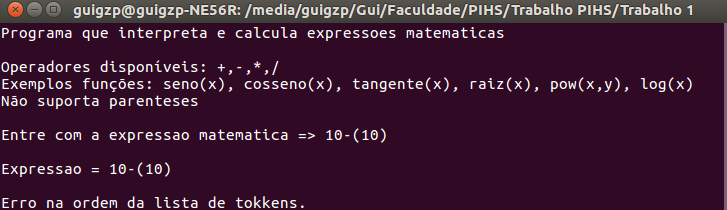
\includegraphics[width=.5\textwidth]{Imagens/erro_parenteses.png}
\caption{Erros Parenteses}
\label{fig:erro_parenteses}
\end{figure}

\item Devido ao não suporte de parênteses, uma expressão da forma 2*(-3) é escrita da forma 2*-3, similarmente, a subtração de um número já negativo ficaria da forma 10--10 que seria equivalente a 10-(-10) como mostra a Figura~\ref{fig:menos};

\begin{figure}[H]
\centering
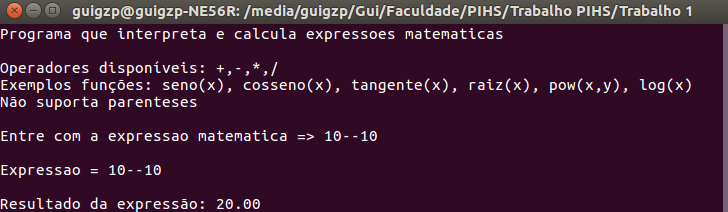
\includegraphics[width=.5\textwidth]{Imagens/dois_menos.png}
\caption{Tratamento para subtração de número negativo}
\label{fig:menos}
\end{figure}

\item Ainda devido a questão deste trabalho não necessitar trabalhar com parênteses, a precedência das operações só depende da sua precedência natural (multiplicação e divisão antes de soma e subtração) e a ordem de aparência na expressão;
\item A expressão deve possui um tamanho máximo de 200 caracteres.
\end{enumerate}

\section*{Conclusão}

O objetivo deste trabalho era implementar um interpretador de expressões matemáticas em linguagem Assembly 32 bits que trabalhasse tanto com  operações básicas quanto algumas mais complexas, sem o tratamento de parênteses.

Através da criação da divisão de tarefas em procedimentos como de leitura da expressão, transformação da expressão para uma lista duplamente encadeada, checagem da lista e redução da lista para um resultado, foi possível atingir o objetivo esperado como mostra a Figura~\ref{fig:resultado} que resolve a expressão ${3^{2} + \sqrt{25}/{5} * {\log_{10} 100} -10 }$.

\begin{figure}[H]
\centering
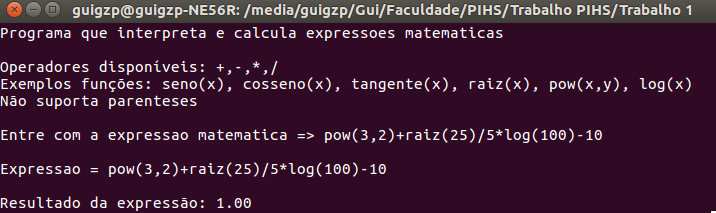
\includegraphics[width=.5\textwidth]{Imagens/resultado.png}
\caption{Resultado de uma expressão}
\label{fig:resultado}
\end{figure}

\nocite{*}

\bibliographystyle{sbc}
\bibliography{Referencias}

\end{document}


